%-------------------------------------------------------------------------------------------------%
% A related work section in which the relevant literature is presented and 
% linked to the project. 
% It should show that you clearly know the problem you plan to solve, 
% and that you master the related work. 
\chapter{Related work}

The introduction already touched upon a number of prior works on the topic of \ac{csg} as well as \ac{wasm}.
However, we are required to examine these studies more closely as well as introduce others, in order to further define our methodology. This study's methodology will draw from prior studies on three topics: The topic of the Geoweb, client-side geoprocessing, and WebAssembly.


\section{Related works on the Geoweb}
% Can't see nothing wrong with it, now that I have pruned it down significantly. Might even be too sharp now, well see. 
\label{sec:geoweb}

The main research question speaks of 'utilization'. Utilization or 'Usability' can mean different things depending on the context used, and which user this applies to. We will define both the type of \emph{usability} and \emph{user} this study speaks of by studying the larger context this study is part of: the Geoweb.

The Geoweb, or Geospatial Web, covers a broad collection of topics located at intersection of the field of geo-information and the web. A noteworthy study on the Geoweb is Van den Brink's phd titled "Geospatial Data on the Web". \cite{brink_geospatial_2018}. She claims that even though geodata is vital to a diverse range of applications and people, the ability to properly retrieve geodata remains almost exclusive to experts in the field. This is to the determent of all these applications and people, jeopardizing value, opportunity, and decision making. She makes this argument by using the concept of FAIR geodata. Coined by \cite{mark_d_wilkinson_fair_2016}, The FAIR principles are a collection of four assessment criteria used to judge the usability of (scientific) data: Findable, Accessible, Interoperable, and Reusable. 

We argue that if these concerns count for geodata \textit{retrieval}, they should just as well count for geodata \textit{processing}. After all, if a user is unable to convert the retrieved geodata to their particular use case, then the information they seek remains inaccessible. Therefore, this study introduces the concept of \emph{FAIR geoprocessing}. 

Based on the arguments presented by \cite{brink_geospatial_2018}, we can also extrapolate that a \ac{gis} environment shouldn't exclusively be used by only experts. Van den Brink mentions a group called 'data users', presented as "web developers, data journalists etc. who use different kinds of data, including geospatial data, directly to create applications or visualizations that supply information to end users (citizens)". 

We use both extrapolations to define the users and 'usability' for the context of this study. We will judge the proposed use case application as 'usable', if it is deemed Findable, Accessible, Interoperable, and Reusable. The user group intended to use this environment is defined as both experts in the field of geo-information and this more general group of data users.

%%%%%%%%%%%%%%%%%%%%%%%%%%%%%%%%%%%%%%%%%%%%%%%%%%%%%%%%%%%%%%%%%%%%%%%%%%%%%%%

\section{Related works on client-side geoprocessing}
% Nothing wrong with this chapter I think. Everything is there for a reason

% the latest in a series of geoprocessing attempts 
% we want to know what happened the previous times, so we will not try things that have already been tried before.

This study will be the latest in a series of studies concerned with client-side geoprocessing. As such, it is important to relate to previous attempts and efforts, to learn from their findings, and to make sure the exact same research will not be performed twice. 

As a side note, client-side geoprocessing is not to be confused with native geoprocessing clients, which would include applications like QGIS \cite{qgis_community_qgis_2022}or ArcGIS \cite{esri_arcgis_2022}. 

Client-side, JavaScript based geoprocessing has seen some level academic interest throughout the last decade. The papers \cite{hamilton_client-side_2014, panidi_hybrid_2015, kulawiak_analysis_2019} all speak of an emergent trend of thick-client websites. Proponents of this trend argue that for certain applications, end users can benefit from dynamic, interactive websites which can immediately respond to a users input, rather than waiting on server round-trips necessary on static web-pages. And by still being a webpage rather than a native application, users can access these applications without installment. The trend is made possible because of hardware improvements of client devices, as well as software improvements, such as HTML5. 

The aforementioned papers each try to apply this trend to the field of geo-informatics. Hamilton et. al. created a such a 'thick-client', capable of replacing certain elements of server-side geoprocessing \cite{hamilton_client-side_2014}. However, the results are unfavorable towards JavaScript. The paper states how "the current implementation of web browsers are limited in their ability to execute JavaScript geoprocessing and not yet prepared to process data sizes larger than about 7,000 to 10,000 vertices before either prompting an unresponsive script warning in the browser or potentially losing the interest of the user.". While these findings are insightful, they are not directly applicable to the efforts of this study proposal. Three reasons for this:

\begin{itemize}
  \item The paper stems from 2014. Since then, web browsers have seen a significant increase in performance thanks to advancements in JavaScript JIT compilers \cite{haas_bringing_2017, kulawiak_analysis_2019}. 
  \item The paper does not use compile-time optimizations. WebAssembly wasn't invented yet, but the authors could have utilized 'asm.js' \cite{mozilla_asmjs_2013} which did exist at the time. 
  \item The paper uses a javascript library which was never designed to handle large datasets.
\end{itemize}

The same statements can be made about similar efforts of Panidi et. al. \cite{panidi_hybrid_2015}. However, Panidi et. al. never proposed client-side geoprocessing as a replacement of server-side geoprocessing, and spend no time on comparing the performance of the two. Instead, the authors propose a hybrid approach, combining the advantages of server-side and client-side geoprocessing. They also present the interesting observation that client-side versus server-side geoprocessing shouldn't necessarily be a compassion of performance. "User convenience" as they put it, might dictate the usage of client-side geoprocessing in certain situations, despite speed considerations \cite{panidi_hybrid_2015}. 

This concern the general web community would label as \ac{ux}, is shared by a more recent paper \cite{kulawiak_analysis_2019}. Their article examines the current state of web-technologies from the point of view of developing cost-effective Web-GIS applications for companies and institutions. Their research reaches a conclusion favorable towards client-side data processing: "[Client-side data processing], in particular, shows new opportunities for cost optimization of Web-GIS development and deployment. The introduction of HTML5 technologies has permitted for construction of platform-independent thick clients which offer data processing performance which under the right circumstances may be close to that of server-side solutions. In this context, institutions [...] should consider implementing Web-GIS with client-side data processing, which could result in cost savings without negative impacts on the user experience.".

% Based on the topic of client-side geospatial processing, we can state that web technologies contain a very dynamic temporal component. All research can become outdated, but performance analysis of web technologies are especially quick to change.  

From these papers we can conclude a true academic and even commercial interest in client-side geoprocessing in the last decade. However, researchers quickly encounter problems during practical implementations in the past. This might not hold up thanks to the recent developments in browser technology, but these papers still show how small, practical implementation details can relate to considerable changes in \ac{ux}. 

Additionally, to the best of the authors's knowledge, all papers concerned with browser-based geoprocessing either tried to use existing JavaScript libraries, or tried to write their own WebAssembly / JavaScript libraries. No studies have been performed on the topic of compiling existing C++ geoprocessing libraries to the web. 

%%%%%%%%%%%%%%%%%%%%%%%%%%%%%%%%%%%%%%%%%%%%%%%%%%%%%%%%%%%%%%%%%%%%%%%%%%%%%%%
\newpage
\section{Related works on WebAssembly}

From all client-side web technologies, WebAssembly is one of the newest, and is most likely to be a deciding factor of this study. This requires us to be aware of the state of WebAssembly, its performance considerations, and how this relates to geoprocessing performance. But first, an introduction on the compilation target itself is in order.

The original paper on WebAssembly was published on June 14, 2017 \cite{haas_bringing_2017}. The authors write that the reason behind the creation of WebAssembly is the observation that certain web applications started using JavaScript as a compile target, using a high-performance subset of JavaScript called 'asm.js' \cite{mozilla_asmjs_2013}. However, JavaScript remains a high-level, highly abstract programming language, which never intended to be used as a compile target. The discrepancy between intended use and actual use led to many complications for developers using JavaScript this way, but also for the developers of JavaScript itself \cite{haas_bringing_2017}. 
In order to relieve javascript of the responsibility of being a 'low-level' compilation target, developers of the four major browser vendors Mozilla, Google, Apple and Microsoft eventually joined up, and created WebAssembly and its corresponding paper.

% This paper starts by promising WebAssembly as a save, fast, portable and compact compilation target. It continues by showing how previous attempts at low-level code on the web fail in at least one of these criteria, and that WebAssembly is the first to deliver on all of them. The follow up chapters cover a proof of memory safety, a proof of soundness of the language design, and the design decisions which had to be made to live up to those four criteria. These details will become relevant to the proposed thesis when reasoning about why WebAssembly might be faster in one case versus another.

\subsection*{Performance}

The initial performance benchmarks look promising. The majority of performance comparisons show that WebAssembly only takes 10\% longer than the native binary it was compared to \cite{haas_bringing_2017}. A later study confirms this by reproducing these benchmarks \cite{jangda_not_2019}. It even notices that improvements have been made in the two years between the studies. However, Jangda et. al. criticize the methodology of these benchmarks, stating that only scientific operations where benchmarked, each containing only 100 lines of code. The paper then continues to show WebAssembly is much more inefficient and inconsistent when it comes to larger applications which use IO operations and contain less-optimized code. These applications turn out to be up to twice as slow compared to native, according to their own, custom benchmarks. Jangda et. al. reason that some of this performance difference will disappear the more mature WebAssembly becomes, but state that WebAssembly has some unavoidable performance penalties as well. One of these penalties is the extra translation step, shown in reffig fig:wasm-trajectory, which is indeed unavoidable when utilizing an in-between compilation target. 

Even though this proposed study falls in the category of scientific computation, these performance considerations will still have to be taken into account. The most important conclusion to to take away from prior research on WebAssembly is that \ac{wasm} must not be regarded as a 'drop-in replacement', as \cite{melch_performance_2019} puts it. Just like any language, WebAssembly has strengths and weaknesses. While \ac{wasm} is designed to be as unassumptious and unopinionated about its source language as possible, the implementations of host environments do favor certain programming patterns and data structures over others, and this will have to be taken into account during the proposed study.

% \begin{figure}[!tbp]
%   \centering
%   \begin{minipage}[b]{0.80\textwidth}
%     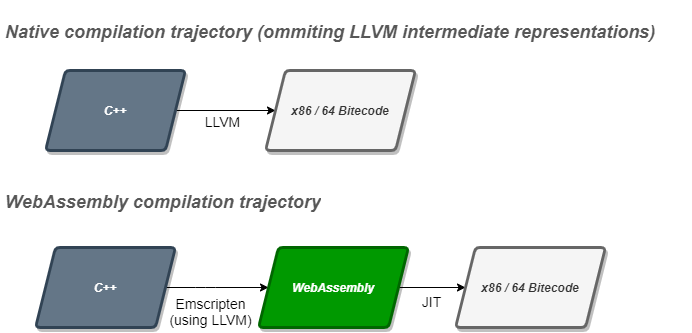
\includegraphics[width=\textwidth]{../schemas/wasm-performance/wasm-perf.png}
%     \caption{Comparison of compilation trajectories}
%     % based on the finding of \cite{jangda_not_2019}
%     \label{fig:wasm-trajectory}
%   \end{minipage}
% \end{figure}

% \subsubsection*{Adoption \& Implementation}

% not in a vaccuum

% On 5 December 2019, the \ac{w3c} officially pronounced WebAssembly as the fourth programming language of the web \cite{w3c_world_2019}. Philippe Le Hégaret, the \ac{w3c} Project Lead, writes “The arrival of WebAssembly expands the range of applications that can be achieved by simply using Open Web Platform technologies. In a world where machine learning and Artificial Intelligence become more and more common, it is important to enable high performance applications on the Web, without compromising the safety of the users,”. Since then, most major browsers have added official WebAssembly support.

% As of writing this proposal, WebAssembly has of yet not seen widespread adoption in web developer communities. Opinions deviate, but in general, WebAssembly is considered a niche technology, often being named as 'experimental' and 'bleeding edge'. 

% This would explain why, to the best of the author's knowledge, not many projects and papers explicitly link WebAssembly and GIS. Papers on \ac{wasm} do state \textit{"3d data transformations and visualization"} as some of the examples of a high performance web applications \cite{haas_bringing_2017, jangda_not_2019}. What's more, certain GIS applications, like Google Earth, have started to use WebAssembly, as seen in \reffig{fig:google-earth} \cite{google_google_2020}. How it is used is unknown due to the engine being closed-source, but it is speculated that \ac{wasm} is used to access code written for the original C++-based desktop application.

% \begin{figure}[!tbp]
%   \centering
%   \begin{minipage}[b]{0.80\textwidth}
%     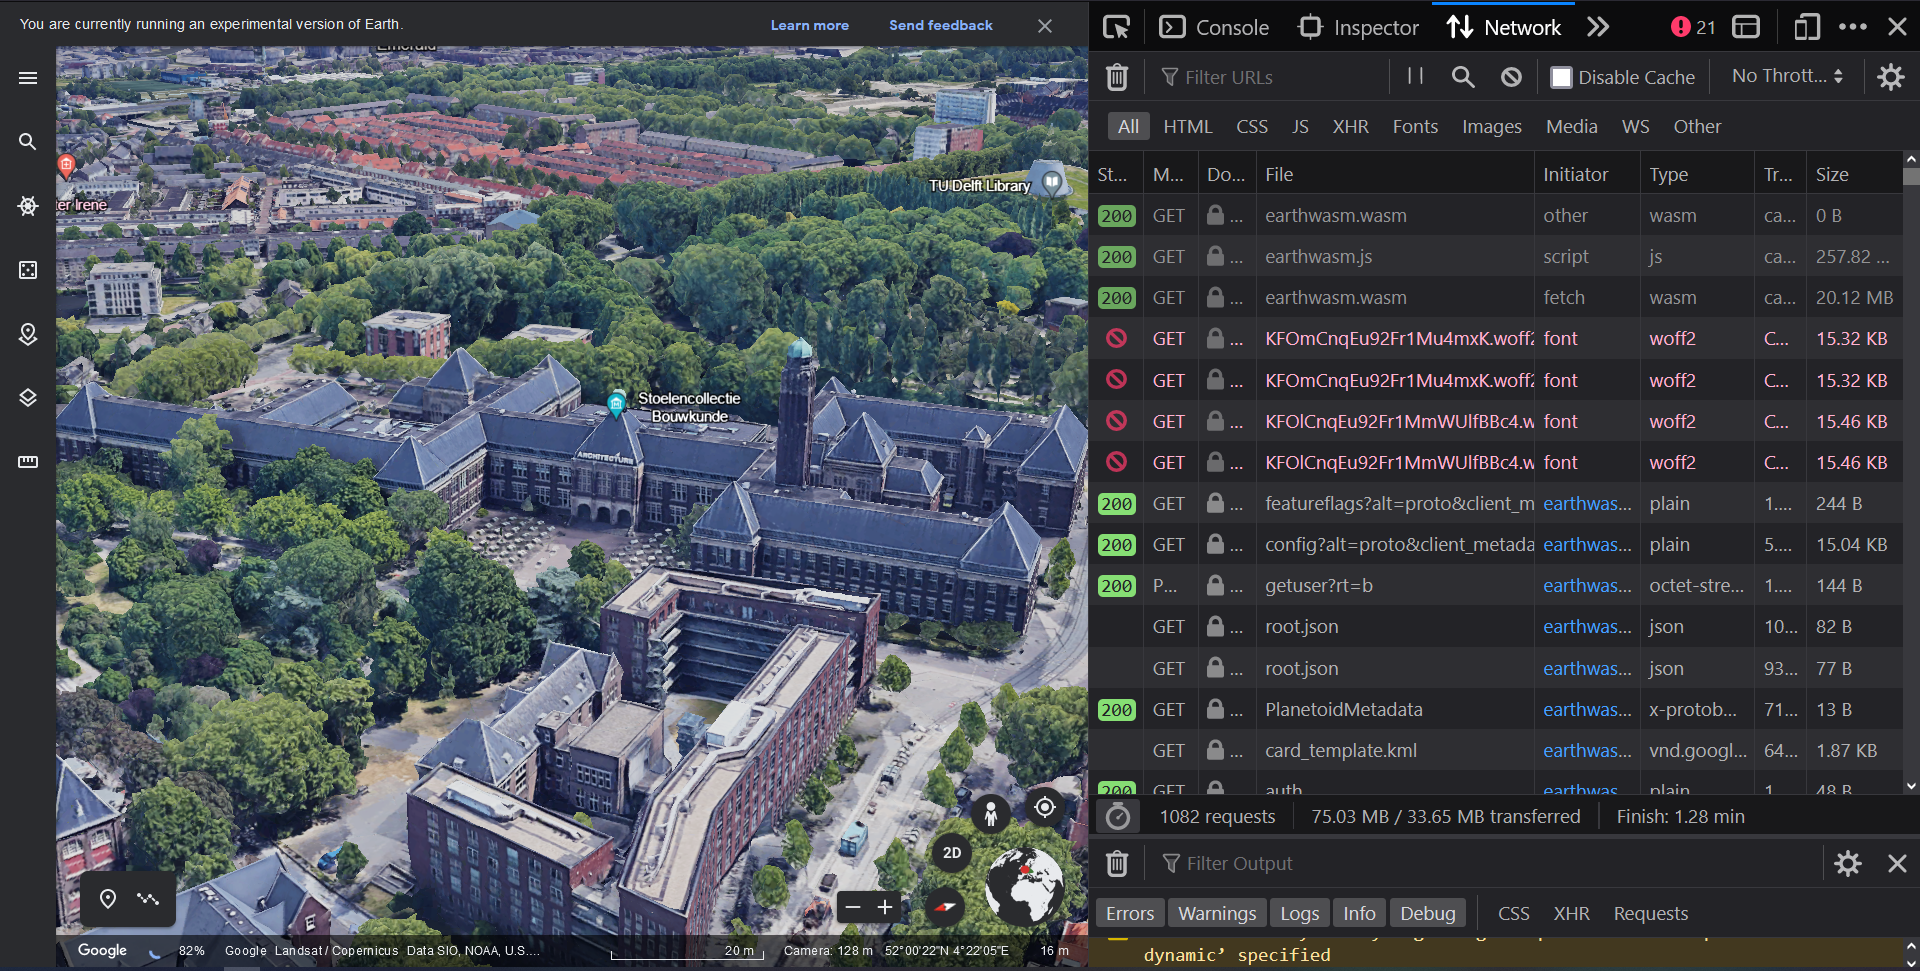
\includegraphics[width=\textwidth]{../images/google-earth-uses-webassembly.PNG}
%     \caption{Google Earth utilizing WebAssembly. Source: \cite{google_google_2020}}
%     \label{fig:google-earth}
%   \end{minipage}
% \end{figure}

% Some studies have taken place evaluating \ac{wasm}'s performance for geospatial operations specifically. Melch performed extensive benchmarks on polygon simplification algorithms written in both javascript and WebAssembly \cite{melch_performance_2019}. It concludes by showing WebAssembly was not always faster, but considerably more consistent. Melch had this to say: "To call the WebAssembly code the coordinates will first have to be stored in a linear memory object. With short run times this overhead can exceed the performance gain through WebAssembly. The pure algorithm run time was always shorter with WebAssembly.". These findings match \cite{jangda_not_2019}, showing that sometimes the javascript JIT compilers of especially the chromium implementation outperform WebAssembly, mainly because of these types of linear memory overhead.

% Lastly, the sparse matrix research of Sandhu et al. will be mentioned. \cite{sandhu_sparse_2018}. It shows again that WebAssembly's performance gain is most notable when performing scientific computations. it states: "For JavaScript, we observed that the best performing browser demonstrated a slowdown of only 2.2x to 5.8x versus C. Somewhat surprisingly, for WebAssembly, we observed similar or better performance as compared to C, for the best performing browser.". It also shows how certain preconceptions must be disregarded during research. For example, it turned out that for WebAssembly and JavaScript, double-precision arithmetic was more performant than single-precision.

% A recent study concerned with watershed delineation \cite{sit_optimized_2019} also concluded client-side WebAssembly to be more performant than server-side C, which, as a side effect, enabled their application to be published on the web. 

% On the topic of WebAssembly, the most important conclusion to to take away from prior research is \ac{wasm} must not be regarded as a 'drop-in replacement', as \cite{melch_performance_2019} puts it. Just like any language, WebAssembly has strengths and weaknesses. While \ac{wasm} is designed to be as unassumptious and unopinionated about its source language as possible, the implementations of host environments do favor certain programming patterns and data structures over others, and this will have to be taken into account during the proposed study.

%%%%%%%%%%%%%%%%%%%%%%%%%%%%%%%%%%%%%%%%%%%%%%%%%%%%%%%%%%%%%%%%%%%%%%%%%%%%%%%
\newpage
\section{Conclusion}

Based on the studies on WebAssembly, we can conclude that the compilation peculiarities of WebAssembly have to be taken into account, as it cannot be regarded as a 'drop in replacement'. There is also a significant difference between using WebAssembly theoretically, and using it realistically. The studies on Client-side geoprocessing tell us that these implementation details can have vast consequences on user experience, and studies on the Geoweb express that this user experience is vital to FAIR, cross-community geoprocessing.

What this means for the methodology, is that a significant portion of this study's attention will have to go to experimenting with different ways of compiling to WebAssembly, while making sure it can still be used in a realistic scenario.
If it turns out that the use-case app can only be used by experienced end-users who take special \ac{wasm} considerations in mind, a big reason of using the web, namely its accessibility, would be lost.  